\documentclass[10pt]{article}
\usepackage{mathpaper}
% \setpreview
\begin{document}
\showsecret
\papertitle{九年级第一学期期末质量检测}
\centerline{\Large 参考答案}
{\centering 注:本答案只给简单过程和评分细则!\par}
\textbf{\selectingintroduction}
\begin{table}[!htb]
    \centering
    \begin{tabularx}{\textwidth}{|*{11}{>{\centering\arraybackslash}X|}} \hline
        题号 & 1 & 2 & 3 & 4 & 5 & 6 & 7 & 8 & 9 & 10 \\ \hline
        选项 & B & D & D & C & D & A & A & C & A & C \\ \hline
    \end{tabularx}
\end{table}

【附解】\setcounter{taskcounter}{9}
\begin{questions}{}
    \question 联立得到$\begin{cases}
        y=tx^2-x \\
        y=4t|x|-t+3
    \end{cases}$,整理得$tx^2-x=4t|x|-t+3$,考虑对此方程进行如下变形:$tx^2-x=4t|x|-t+3 \Rightarrow tx^2-4t|x|+t=x+3 \Rightarrow t\left(x^2-4|x|+1\right)=x+3$,考虑令$k=\frac{1}{t}$,那么原方程又可化为$x^2-4|x|+1=k(x+3)$,这可以看成是$y=x^2-4|x|+1$与$y=k(x+3)$联立,在同一直角坐标系作出图像:\par
    \begin{figure}[!htb]
        \centering
        \begin{tikzpicture}[>=Stealth,scale=0.5]
            \draw[->] (-7,0) -- (3,0) node[below] {$x$};
            \draw[->] (0,-4) -- (0,7) node[right] {$y$};
            \draw (-5,6) parabola bend (-2,-3) (0,1);
            \draw (0,1) parabola bend (2,-3) (2,-3);
            \draw[densely dashed] (-5,7) -- (-5,-4);
            \draw[densely dashed] (1,7) -- (1,-4);
            % \node[below] at (-5,0) {$-5$};
            % \node[below] at (1,0) {$1$};
            \draw (-3,0.2) -- (-3,0) node[below] {$-3$};
            \draw[densely dashed] (-16/3,7) -- (-5/3,-4) node[below] {$k=-3$};
            \draw[densely dashed] (-6,3/2) -- (4,-7/2) node[below] {$k=-\frac{1}{2}$};
            \draw[densely dashed] (-6,-1) -- (3,2) node[right] {$k=\frac{1}{3}$};
        \end{tikzpicture}
        \caption*{(第10题图解)}
    \end{figure}
    从图像上可以看出,当$-3 \leq k < -\frac{1}{2}$或$k=\frac{1}{3}$时,原方程有两组解,对应可得$t$的取值范围是$-2 < t \leq -\frac{1}{3}$或$t=3$,其中,整数只有$-1$和$3$这$2$个,故选C.
\end{questions}

\par \textbf{\complitingintroduction}
\begin{table}[!htb]
    \centering
    \renewcommand\arraystretch{1.5}
    \begin{tabularx}{\textwidth}{*{3}{>{\centering\arraybackslash}X}}
        11.$-1$ & 12.$106^{\circ}$或$164^{\circ}$ & 13.$108$ \\
        14.$2$或$-\frac{5}{2}$ & 15.\circnum{1}\circnum{3}\circnum{4} & 16.$2\sqrt{3}$  \\
    \end{tabularx}
\end{table}

\setcounter{taskcounter}{16}
\begin{questions}{\answeringintroduction}
    \question 由二次根式的非负性知$a=2$、$b=-3$\point{3},由根的定义知$a+b+c=0$,代入得到$c=1$\point{5},于是原方程化为$\frac{1}{4}y^2-1=0$,据此解得$y_1=-2$、$y_2=2$\point{8}.
    \question
    \begin{subquestions}
        \subquestion 证明$\triangle ABE$和$\triangle ACF$全等就可得到$\triangle AEF$是等边三角形.\point{4}

        % \begin{figure}[!htb]
        %     \raggedleft
        %         \begin{tikzpicture}[scale=0.45]
        %             \coordinate[label=above:{$A$}] (A) at (3,5.19615);
        %             \coordinate[label=below left:{$B$}] (B) at (0,0);
        %             \coordinate[label=below right:{$C$}] (C) at (6,0);
        %             \coordinate[label=below:{$E$}] (E) at (2,0);
        %             \coordinate[label=right:{$F$}] (F) at (7,1.73205);
        %             \draw (A) -- (B) -- (C) -- cycle;
        %             \draw (A) -- (E) -- (F) -- cycle;
        %             \draw (C) -- (F);
        %         \end{tikzpicture}
        % \end{figure}
        \subquestion 过$E$作$ET \bot CF$交$FC$延长线于$T$,易证$CT=1$、$ET=\sqrt{3}$,于是$S_{\triangle ECF}=\frac{1}{2}ET \cdot CF=\frac{\sqrt{3}}{2}$.\point{8}
    \end{subquestions}
    \question %19
    \begin{subquestions}
        \subquestion $\frac{11}{16}$\point{3}
        \subquestion 由树状图(表格)\point{5}可知有$12$种等可能的结果\point{6},其中``两球标号互质''共$4$种\point{7},故$P(\text{两球标号互质})=\frac{4}{12}=\frac{1}{3}$.\point{8}
    \end{subquestions}
    \question %20
    \begin{subquestions}
        \subquestion $\wideparen{DB^l}=\frac{\pi}{3}$\point{1}、$S=\pi - 2$\point{2}
        \subquestion 在$CD$延长线上截$TD=BD$,连$AT$,证明$\triangle TAD$与$\triangle BAD$全等\point{5},再证$\triangle TAC$是等腰直角三角形,得到$BD+DC=TD+DC=TC=\sqrt{2}AC=2\sqrt{6}$即可\point{8}.
        \begin{figure}[!htb]
            \raggedleft
                \begin{tikzpicture}[scale=0.475]
                    \coordinate[label=above:{$A$}] (A) at (3,5.19615);
                    \coordinate[label=below left:{$B$}] (B) at (0,0);
                    \coordinate[label=below right:{$C$}] (C) at (6,0);
                    \coordinate[label=below left:{$D$}] (D) at (-0.46410,1.73205);
                    \coordinate[label=below right:{$O$}] (O) at (3,1.73205);
                    \draw (A) -- (B) -- (C) -- cycle;
                    \filldraw (O) circle (0.05);
                    \draw (O) circle (3.46410);
                    \draw (A) -- (D);
                    \draw (B) -- (D);
                    \draw (C) -- (D);
                    \coordinate[label=above:{$T$}] (T) at (-2.19615,2.19615);
                    \draw[ansline] (A) -- (T) -- (D);
                \end{tikzpicture}
        \end{figure}
    \end{subquestions}
    \question \textcolor{blue}{作出$AD$给2分,作出点$E$给5分,作出$AF$给8分}
    \begin{figure}[!htb]
        \raggedleft
            \begin{tikzpicture}[scale=0.7]
                \draw[step=1,dashed] (-1,-2) grid (6,5);
                \coordinate[label=below right:{$C$}] (C) at (4,0);
                \coordinate[label=above left:{$A$}] (A) at (0,3.28083);
                \coordinate[label=below left:{$B$}] (B) at (0,0);
                \coordinate (O) at (2,1.64042);
                \draw (O) circle (2.58669);
                \draw (B) -- (A) -- (C);
                \coordinate[label=below:{$D$}] (D) at (2,-0.94627);
                \draw[ansline] (B) -- (4,4);
                \draw[ansline,blue] (A) -- (D) -- (B);
                \coordinate[label=above:{$E$}] (E) at (1.05373,1.05373);
                \draw[ansline] (3.38418,4.56595) -- (0.50892,-1.51106);
                \coordinate[label=below right:{$F$}] (F) at (4.53670,1.13435);
                \draw[ansline] (B) -- (F);
                \draw[ansline,blue] (A) -- (F);
            \end{tikzpicture}
    \end{figure}
    \question %22
    \begin{subquestions}
        \subquestion $v_1=-20t_1+40$\point{1}、$s=-10t^2+40t$\point{2}
        \subquestion 由小球乙共运动$3$秒可知当$t_2=3$时,$h=0$\point{3},进而解得$v_2=6$\point{4}.从而$v_1=v_2=6$,对应可解得$t_1=1.7$\point{5},代入$s$得到$s=39.1$,故$AB$长$39.1$dm\point{6}.
        \subquestion 解三角形得到$h_{max}=2$\point{7},分析$h-v_2$图像可得当$t_2=\frac{v_2}{4}$时,$h=2$,解方程并舍去负根得到$v_2=4$\point{8},从而$v_1=v_2=4$,对应可解得$t_1=1.8$\point{9},代入$s$得到$s=39.6$,故$AB$长$39.6$dm\point{10}.
        % \begin{figure}[!htbp]
        %     \raggedleft
        %     \begin{tikzpicture}[scale=0.45,>=Stealth]
        %         \draw (-7,0) -- (10,0);
        %         \draw (3,5) -- (9,5);
        %         \coordinate (B) at (4,1);
        %         \coordinate (D) at (7.46410,3);
        %         \node[above right] at (8.14711,3) {$D$};
        %         \node[above right] at (4.25,0.75) {$B$};
        %         \coordinate[label=above:{$O$}] (O) at (4,5);
        %         \draw (B) -- (O);
        %         \draw[densely dashed] (O) -- (D);
        %         \draw (4,0.5) circle (0.5);
        %         \draw (-5,0.5) circle (0.5);
        %         \node[above right] at (-4.75,0.75) {$A$};
        %         \draw[densely dashed] (7.89711,2.75) circle (0.5);
        %         \draw[densely dashed] (0,0.5) circle (0.5);
        %         \draw[->] (-3.6,1.1) -- (-2.6,1.1) node[above left] {$v_1$};
        %         \draw[densely dashed] (2.3,2.75) -- (7.5,2.75);
        %         \node[left] at (2.5,1.375) {$h$};
        %         \draw[<->] (2.5,0.1) -- (2.5,2.74);
        %         \draw[densely dashed] (4,0.5) arc (270:330:4.5);
        %     \end{tikzpicture}
        % \end{figure}
    \end{subquestions}
    \question %23
    \begin{subquestions}
        \subquestion 直接导角即可\point{2}.
        \begin{figure}[!htb]
            \raggedleft
            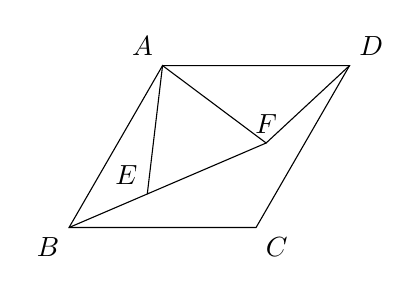
\begin{tikzpicture}[scale=0.475]
                \coordinate[label=above left:{$A$}] (A) at (2.5,4.33013);
                \coordinate[label=below left:{$B$}] (B) at (0,0);
                \coordinate[label=below right:{$C$}] (C) at (5,0);
                \coordinate[label=above right:{$D$}] (D) at (7.5,4.33013);
                \draw (A) -- (B) -- (C) -- (D) -- cycle;
                \coordinate[label=above left:{$E$}] (E) at (2.09151,0.89705);
                \coordinate[label=above:{$F$}] (F) at (5.26889,2.25983);
                \draw (A) -- (E) -- (F) -- cycle;
                \draw (B) -- (E);
                \draw (D) -- (F);
            \end{tikzpicture}
        \end{figure}
        \subquestion 连$EC$、$AC$,证明$\triangle ADC$是等边三角形\point{3},从而得到$\triangle AEC$全等于$\triangle AFD$\point{5},于是$\angle ECA=\angle FDA$、$EC=DF$,这可以得到$\angle BEC=135^{\circ}$\point{6},最后解$\triangle BEC$就可以得到$BE=2$\point{7}.
        \begin{figure}[!htb]
            \raggedleft
            \begin{tikzpicture}[scale=0.475]
                \coordinate[label=above left:{$A$}] (A) at (2.5,4.33013);
                \coordinate[label=below left:{$B$}] (B) at (0,0);
                \coordinate[label=below right:{$C$}] (C) at (5,0);
                \coordinate[label=above right:{$D$}] (D) at (7.5,4.33013);
                \draw (A) -- (B) -- (C) -- (D) -- cycle;
                \coordinate[label=above left:{$E$}] (E) at (3.17839,0.96984);
                \coordinate[label=above:{$F$}] (F) at (5.74929,3.23749);
                \draw (A) -- (E) -- (F) -- cycle;
                \draw (B) -- (E);
                \draw (D) -- (F);
                \draw[ansline] (E) -- (C) -- (A);
            \end{tikzpicture}
        \end{figure}
        \subquestion $PQ_{min}=\sqrt{35}-3$\point{10}.
    \end{subquestions}
    \question %24
    \begin{subquestions}
        \subquestion
        \begin{subsubquestions}
            \subsubquestion $(0,1)$\point{1} ;$(-2,2)$或$(2,2)$\point{2}
            \subsubquestion $y=\frac{1}{4}x^2+1$\point{3}
        \end{subsubquestions}
        \subquestion \textbf{【解答】} \par
        \begin{figure}[!htb]
            \raggedleft
            \begin{tikzpicture}[>=Stealth,scale=0.5]
                \draw[->] (-4.25,0) -- (4.25,0) node[below] {$x$};
                \draw[->] (0,-1) -- (0,5.5) node[right] {$y$};
                \coordinate[label=below right:{$O$}] (O) at (0,0);
                \draw (-4,5) parabola bend (0,1) (4,5);
                \coordinate[label=below left:{$P$}] (P) at (-2,2);
                \coordinate[label=below left:{$M$}] (M) at (-3.75078,4.51710);
                \coordinate[label=below right:{$N$}] (N) at (2.56938,2.65043);
                \draw (P) -- (M) -- (N) -- cycle;
                \coordinate[label=above right:{$C$}] (C) at (-2,4);
                \draw[ansline] (-2,0.5) -- (-2,4.75);
            \end{tikzpicture}
        \end{figure}
        如图,过$P$作$PC \bot x\text{轴}$交$MN$于$C$. \par
        $\because x_P=-2$、$MN:y=kx+2k+4$.$\therefore P(-2,2)$、$C(-2,4) \Rightarrow PC=x_C-x_P=2$\point{4}. \par
        联立$MN$和$\Gamma$的方程可得到$\begin{cases}
            y=\frac{1}{4}x^2+1 \\
            y=kx+2k+4
        \end{cases}$,整理得$x^2-4kx-8k-12=0$.由于$x_M$、$x_N$是这个方程的两根,故由韦达定理,$\begin{cases}
            x_M+x_N=4k \\
            x_M \cdot x_N = -8k-12
        \end{cases}$\point{6}.\par
        令$h=(x_M-x_N)^2$,有$S_{\triangle MPN}=\frac{1}{2}PC\sqrt{h}=\sqrt{h}$,故当$S_{\triangle MPN}$最小时,$h$最小.\par
        $\because h=(x_M-x_N)^2=(x_M+x_N)^2-4x_M \cdot x_N=16k^2+32k+48=16(k+1)^2+32$,$\therefore$当$k=-1$时,$h$取最小值$32$,$\therefore$当$k=-1$时,$S_{\triangle MPN}$取到最小值$4\sqrt{2}$.\par
        综上所述,$\triangle MPN$的面积最小为$4\sqrt{2}$.\point{8}
        \subquestion \textbf{【解答】} \par
        \textbf{【点参法】} \par
        \begin{figure}[!htb]
            \raggedleft
            \begin{tikzpicture}[>=Stealth,scale=0.5]
                \draw[->] (-4.25,0) -- (4.25,0) node[below] {$x$};
                \draw[->] (0,-1) -- (0,5.5) node[right] {$y$};
                \coordinate[label=below right:{$O$}] (O) at (0,0);
                \coordinate[label=right:{$F$}] (F) at (0,2);
                \draw (-4,5) parabola bend (0,1) (4,5);
                \coordinate[label=below left:{$P$}] (P) at (-3,3.25);
                \coordinate[label=below right:{$Q$}] (Q) at (1.333333,1.444444);
                \coordinate[label=below:{$T$}] (T) at (-0.83333,0);
                \draw (P) -- (Q) -- (T) -- cycle;
                \draw (F) -- (T);
            \end{tikzpicture}
        \end{figure}
        设$P(2p,p^2+1)$、$Q(2q,q^2+1)$、$PQ:y=k'x+b'$、$PT:y=mx+n$. \par
        这样有$\begin{cases}
            p^2+1=2pk'+b' \\
            q^2+1=2qk'+b'
        \end{cases}$,解得$\begin{cases}
            k'=\frac{p+q}{2} \\
            b'=-pq
        \end{cases}$,故$PQ:y=\frac{p+q}{2}x-pq$,又$\because PQ$过$F(0,2)$.$\therefore -pq=2 \Rightarrow pq=-2$\point{9} \par
        $\because P$在$PT$上.$\therefore p^2+1=2mp+n \Rightarrow n=-2pm+p^2+1 \Rightarrow PQ:y=mx-2pm+p^2+1$\par
        联立$PT$和$\Gamma$的方程,有$\begin{cases}
            y=\frac{1}{4}x^2+1 \\
            y=mx-2pm+p^2+1
        \end{cases}$,整理得$x^2-4mx+8pm-4p^2=0$.$\because PT$与$\Gamma$有且仅有一个公共点.$\therefore$此方程两实根相同,即
        $$\begin{aligned}
            \Delta = 0 \Rightarrow (-4m)^2-4(8pm-4p^2) &= 0 \\
            m^2-2pm+p^2 &= 0 \\
            (m-p)^2 &= 0 \\
            m &= p
        \end{aligned}$$
        故$PT:y=px-p^2+1$,同理,$QT:y=qx-q^2+1$\point{11}. \par
        联立$PT$和$QT$的方程,有$\begin{cases}
            y=px-p^2+1 \\
            y=qx-q^2+1
        \end{cases}$,解得$\begin{cases}
            x=p+q \\
            y=pq+1=0
        \end{cases}$,即$T(p+q,0)$.\par
        $\because$由勾股定理,
        $$\begin{aligned}
            PF^2 &= (x_P-x_F)^2+(y_P-y_F)^2 = 4p^2+(p^2-1)^2 = (p^2+1)^2 \\
            FT^2 &= (x_F-x_T)^2+(y_F-y_T)^2 = (p+q)^2+4 = (p+q)^2-4pq = (p-q)^2 \\
            PT^2 &= (x_P-x_T)^2+(y_P-y_T)^2 = (p-q)^2+(p^2+1)^2 = PF^2+FT^2
        \end{aligned}$$
        $\therefore$由勾股逆定理,$TF \bot PQ$,证毕.\point{12}
        \par \textbf{【线参法】} \par
        \begin{figure}[!htb]
            \raggedleft
            \begin{tikzpicture}[>=Stealth,scale=0.5]
                \draw[->] (-4.25,0) -- (4.25,0) node[below] {$x$};
                \draw[->] (0,-1) -- (0,5.5) node[right] {$y$};
                \coordinate[label=below right:{$O$}] (O) at (0,0);
                \coordinate[label=right:{$F$}] (F) at (0,2);
                \draw (-4,5) parabola bend (0,1) (4,5);
                \coordinate[label=below left:{$P$}] (P) at (-3,3.25);
                \coordinate[label=below right:{$Q$}] (Q) at (1.333333,1.444444);
                \coordinate[label=below:{$T$}] (T) at (-0.83333,0);
                \draw (P) -- (Q) -- (T) -- cycle;
                \draw (F) -- (T);
                \coordinate[label=above:{$C$}] (C) at (-0.83333,2.34722);
                \draw[ansline] (C) -- (T);
            \end{tikzpicture}
        \end{figure}
        设$PQ:y=kx+b$,$\because PQ$过$F(0,2)$.$\therefore 2=b \Rightarrow b=2 \Rightarrow PQ:y=kx+2$ \par
        联立$PQ$和$\Gamma$的方程,有$\begin{cases}
            y=\frac{1}{4}x^2+1 \\
            y=kx+2
        \end{cases}$,整理得$x^2-4kx-4=0$.$\because x_P$、$x_Q$是这个方程的两根.$\therefore$由韦达定理,$\begin{cases}
            x_P+x_Q=4k \\
            x_P \cdot x_Q=-4
        \end{cases}$ \point{9} \par
        设$T(p,q)$,过$T$的直线$l_T:y=mx+n$,有$q=mp+n \Rightarrow n=-mp+q \Rightarrow l_T:y=mx-mp+q$.\par
        联立$l_T$和$\Gamma$的方程,有$\begin{cases}
            y=\frac{1}{4}x^2+1 \\
            y=mx-mp+q
        \end{cases}$,整理得$x^2-4mx+4mp-4q+4=0$\par
        当$l_T$与$\Gamma$有且仅有一个公共点时,此方程两实根相同,即
        $$\begin{aligned}
            \Delta = 0 \Rightarrow (-4m)^2-4(4mp-4q+4) &= 0 \\
            m^2-mp+q-1 &= 0
        \end{aligned}$$
        由韦达定理,$\begin{cases}
            m_1+m_2=p \\
            m_1 \cdot m_2 = q-1
        \end{cases}$,此时方程的解为$x_1=x_2=2m$,故可设$PT:y=m_1x-m_1p+q$、$QT:y=m_2x-m_2p+q$,有$x_P=2m_1$、$x_Q=2m_2$\point{11}. \par
        于是$\begin{cases}
            2m_1+2m_2=4k \\
            2m_1 \cdot 2m_2 = -4
        \end{cases} \Rightarrow \begin{cases}
            2p=4k \\
            q-1=-1
        \end{cases} \Rightarrow \begin{cases}
            p = 2k \\
            q = 0
        \end{cases} \Rightarrow T(2k,0)$ \par
        如图,过$T$作$TC \bot x\text{轴}$交$PQ$于$C$,则$C(2k,2k^2+2)$,故$CT=y_C-y_T=2k^2+2 \Rightarrow CT^2=4k^4+8k^2+4$ \par
        $\because$由勾股定理,
        $$\begin{aligned}
            CF^2 &= (x_C-x_F)^2+(y_C-y_F)^2 = (2k)^2+(2k^2+2-2)^2 = 4k^4+4k^2 \\
            TF^2 &= (x_T-x_F)^2+(y_T-y_F)^2 = (2k)^2+(2)^2 = 4k^2+4
        \end{aligned}$$
        $\therefore CT^2=CF^2+TF^2$,由勾股逆定理,$PQ \bot TF$,证毕.\point{12}
    \end{subquestions}
\end{questions}
\end{document}